\begin{example}
  [The Abstract Control Flow Graph for Two Paths Loop and Nested Loop in One Path]
  \label{ex:relatedNestedWhileOdd_abscfg}
    { \small
  \begin{figure}
  \centering
  \begin{subfigure}{.4\textwidth}
    \begin{centering}
    {\small
    $
    \begin{array}{l}
      \kw{relatedNestedWhileOdd}(n, m) \triangleq \\
      \clabel{ \assign{i}{n} }^{0} ; \\
          \ewhile ~ \clabel{i > 0}^{1} ~ \edo ~ \\
          \qquad \Big(
            \eif(\clabel{i \% 2 \neq 0 }^{2},\\
            \qquad \clabel{\assign{k}{i - m}}^{3};\\
            \qquad \ewhile ~ \clabel{k > 0}^{4} ~ \edo ~
            \Big( \clabel{\assign{k}{k - 1}}^{5} \Big);\\
            \qquad \clabel{\assign{i}{k + m}}^{6};
            \clabel{\assign{i}{i - 1}}^{7}, \\
            \qquad \clabel{\assign{i}{i - 3}}^{8})
            \Big)
      \end{array}
    $
    }
    \caption{}
    \end{centering}
    \end{subfigure}
  \begin{subfigure}{.5\textwidth}
    \begin{centering}
  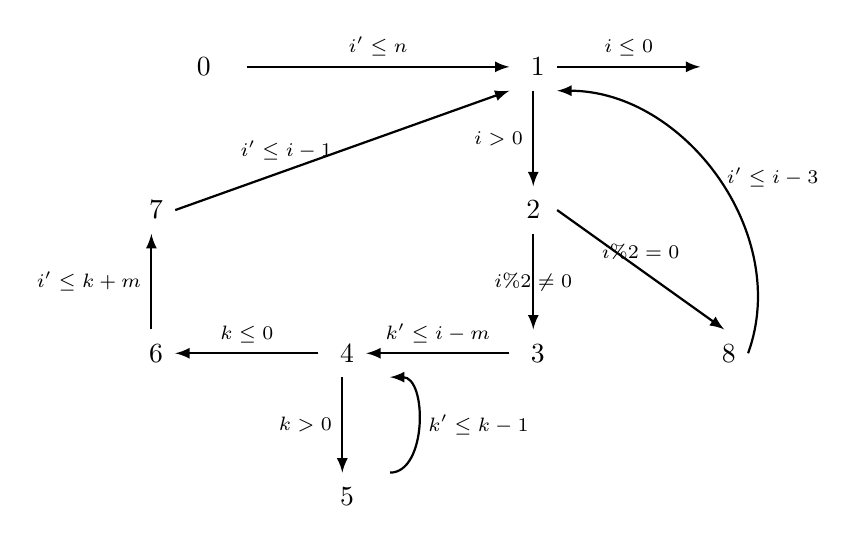
\begin{tikzpicture}[scale=\textwidth/20cm,samples=200]
  \draw[] (-7, 10) circle (0pt) node{{ $0$}};
  \draw[] (0, 10) circle (0pt) node{{ $1$}};
  \draw[] (0, 7) circle (0pt) node{\textbf{$2$}};
  \draw[] (0, 4) circle (0pt) node{{ $3$}};
  \draw[] (-4, 4) circle (0pt) node{{ $4$}};
  \draw[] (-8, 4) circle (0pt) node{{ $6$}};
  \draw[] (-4, 1) circle (0pt) node{{ $5$}};
  \draw[] (4, 4) circle (0pt) node{{ $8$}};
  \draw[] (-8, 7) circle (0pt) node{{ $7$}};
  % Counter Variables
  \draw[] (4.5, 10) circle (0pt) node {\textbf{$\lex$}};
  % \draw[] (6, 4) circle (0pt) node {{ $ex$}};
  %
  % Control Flow Edges:
  \draw[ thick, -latex] (-6, 10)    -- node [above] {\scriptsize $i' \leq n$}(-0.5, 10);
  \draw[ thick, -latex] (0, 9.5)    -- node [left] {\scriptsize $i > 0$} (0, 7.5) ;
  \draw[ thick, -latex] (0.5, 7)    -- node [above] {\scriptsize $ i \% 2 = 0 $}  (4, 4.5);
  \draw[ thick, -latex] (4.5, 4)    to  [out=70,in=0]   node [right] {\scriptsize $i' \leq i - 3$ }(0.5, 9.5);
  \draw[ thick, -latex]  (0, 6.5)   -- node  {\scriptsize $i \% 2 \neq 0$}  (0, 4.5) ;
  \draw[ thick, -latex]  (-0.5, 4)  -- node [above] {\scriptsize $k' \leq i - m$ }  (-3.5, 4) ;
  \draw[ thick, -latex]  (-4.5, 4)  -- node [above] {\scriptsize $k \leq 0$ }  (-7.5, 4);
  \draw[ thick, -latex] (0.5, 10)   -- node [above] {\scriptsize $i \leq 0$}  (3.5, 10);
  \draw[ thick, -latex] (-4, 3.5)   -- node [left] {\scriptsize $k > 0$}  (-4, 1.5);
  \draw[ thick, -latex] (-3, 1.5)   to  [out=0,in=0] node [right] {\scriptsize $k' \leq k- 1$}  (-3, 3.5);
  \draw[ thick, -latex] (-8, 4.5)   --  node [left] {\scriptsize $i' \leq k + m$ }(-8, 6.5);
  \draw[ thick, -latex] (-7.5, 7)  --  node [left] {\scriptsize $i' \leq i - 1$ }(-0.5, 9.5);
  % \draw[ thick, -latex] (6, 6.5)  -- node [right] {$\top$} (6, 4.5) ;
  \end{tikzpicture}
  \caption{}
    \end{centering}
    \end{subfigure}
  \caption{
  (a) The program of the two paths loop with a nested Loop in one path,
    (b) The corresponding \emph{Abstract Execution Control Flow Graph}, $\absG(\kw{relatedNestedWhileOdd}(n, m))$. }
      \label{fig:relatedNestedWhileOdd_abscfg}
  \end{figure}
  }
  %
  The program in Figure~\ref{fig:relatedNestedWhileOdd_abscfg}(a) is an example of two paths loop with different reachability-bounds on the control
locations in different paths.
Its abstract control flow graph is shown in Figure~\ref{fig:relatedNestedWhileOdd_abscfg}(b).
The edge $(0 \xrightarrow{i' \leq n} 1)$ on the top tells us the command 
$\clabel{\assign{i}{n}}^0$ is executed with a continuation point $1$, and the
command $\ewhile \clabel{i > 0}^1 \edo \{\ldots\}$ will be executed next.
The annotation $i' \leq n$ is a difference constraint 
computed by $\absexpr$ over
the expression $n$ in the assignment command $\assign{i}{n}$.
It represents that the value of $i$ is less than or equal to value of $n$ after the
execution of $\clabel{\assign{i}{n}}^0$ and before evaluating the guard $\clabel{i > 0}^1$.
Another example constraint $i' \leq i - 1$ on the edge $7 \xrightarrow{i' \leq i - 1} 1$
describes the execution of
 the command at line $7$, 
$\clabel{\assign{i}{i - 1}}^{7}$. 
The $i'$ on the left side of $i' \leq i - 1$ represents the value of $i$ after the assignment operation,
and the right-hand side $i$ stores the value before the assignment.
The boolean constraint $i \leq 0 $ on the edge $1 \xrightarrow{i \leq 0} \lex$, 
represents the negation of the testing guard $\clabel{i > 0}^1$
in the $\ewhile$ command.
$1 \xrightarrow{i \leq 0} \lex$ denotes that $i \leq 0$ must hold in order to perform this transition from program point $1$ to
the program exit. 
  \end{example}    
  